% CoMemTree pipeline figure (full-width, WWW / ACM sigconf: \textwidth = 7in = 17.8cm)
% Compile: xelatex pipeline.tex  (Libertinus = open Libertine/Biolinum clone, matches acmart)
%      or: pdflatex pipeline.tex (falls back to libertine + newtxmath, as in acmart)
% Use in paper:  \begin{figure*}\includegraphics[width=\textwidth]{figures/pipeline.pdf} ... \end{figure*}
\documentclass[10pt,border=1pt]{standalone}
\usepackage{iftex}
\ifXeTeX
  \usepackage{amsmath,amssymb}
  \usepackage{unicode-math}
  \setmainfont{Libertinus Serif}
  \setsansfont{Libertinus Sans}
  \setmathfont{Libertinus Math}
\else
  \usepackage{amsmath,amssymb}
  \usepackage[T1]{fontenc}
  \usepackage{libertine}
  \usepackage[libertine]{newtxmath}
\fi
\usepackage{tikz}
\usetikzlibrary{positioning,calc,arrows.meta,shapes.geometric,backgrounds,fit,decorations.pathreplacing}
\renewcommand{\familydefault}{\sfdefault}

% ---------------- palette ----------------
\definecolor{ink}{HTML}{2B2F36}
\definecolor{mute}{HTML}{6B7280}
\definecolor{rule}{HTML}{C9CED6}
\definecolor{panel}{HTML}{F7F8FA}
\definecolor{band}{HTML}{E9ECF1}
\definecolor{what}{HTML}{1F5FAD}   \definecolor{whatbg}{HTML}{DCE8F6}
\definecolor{how}{HTML}{D2691E}    \definecolor{howbg}{HTML}{FBE5D2}
\definecolor{llm}{HTML}{5E4FA2}    \definecolor{llmbg}{HTML}{ECE8F7}
\definecolor{stay}{HTML}{2A8C82}   \definecolor{staybg}{HTML}{DDF1EE}
\definecolor{histbg}{HTML}{EEF0F3}
% behavior-state colours (s1..s4)
\definecolor{sA}{HTML}{3E9C8C}
\definecolor{sB}{HTML}{C9A227}
\definecolor{sC}{HTML}{C05A7A}
\definecolor{sD}{HTML}{6E8B3D}
% item colours (generic categories)
\definecolor{iA}{HTML}{B9C7DA}\definecolor{iB}{HTML}{D9C9B4}\definecolor{iC}{HTML}{C7D6C2}\definecolor{iD}{HTML}{D6C3D3}

\newcommand{\tsz}{\fontsize{6}{7}\selectfont}       % small annotation text (6pt)
\newcommand{\lsz}{\fontsize{7}{8.2}\selectfont}     % label text (7pt)
\newcommand{\hsz}{\fontsize{8}{9.5}\selectfont}     % panel titles (8pt)

\tikzset{
  >={Stealth[length=4pt,width=3.2pt]},
  flow/.style={->,line width=0.7pt,draw=ink},
  panelbox/.style={draw=rule,fill=panel,rounded corners=3pt,line width=0.5pt},
  item/.style={rectangle,rounded corners=1pt,minimum size=0.21cm,inner sep=0pt,draw=ink!45,line width=0.3pt},
  win/.style={draw=mute,dashed,rounded corners=2pt,line width=0.45pt},
  st/.style={circle,minimum size=0.33cm,inner sep=0pt,text=white,font=\tsz\bfseries,draw=white,line width=0.4pt},
  chip/.style={rectangle,rounded corners=2pt,minimum height=0.30cm,inner sep=1.5pt,font=\tsz},
  slot/.style={rectangle,rounded corners=2pt,minimum width=4.55cm,inner sep=2.5pt,align=left,anchor=west,font=\lsz,line width=0.5pt},
}

% state node: \st{name}{(x,y)}{colour}{index}
\newcommand{\st}[4]{\node[st,fill=#3] (#1) at #2 {#4};}
% snowflake (frozen model)
\newcommand{\snow}[2]{%
  \begin{scope}[shift={#1},line width=0.55pt,draw=#2,line cap=round]
    \foreach \a in {90,150,210,270,330,30}{
      \draw (0,0) -- (\a:0.13);
      \draw (\a:0.085) -- ++(\a+40:0.04);
      \draw (\a:0.085) -- ++(\a-40:0.04);
    }
  \end{scope}}
% mini histogram over 4 states, heights h1..h4 (cm), origin (x,y)
\newcommand{\hist}[6]{%
  \begin{scope}[shift={#1}]
    \fill[sA] (0,0) rectangle ++(#6,#2);
    \fill[sB] (#6*1.35,0) rectangle ++(#6,#3);
    \fill[sC] (#6*2.7,0) rectangle ++(#6,#4);
    \fill[sD] (#6*4.05,0) rectangle ++(#6,#5);
    \draw[ink!60,line width=0.3pt] (-0.03,0) -- (#6*5.1,0);
  \end{scope}}

\begin{document}
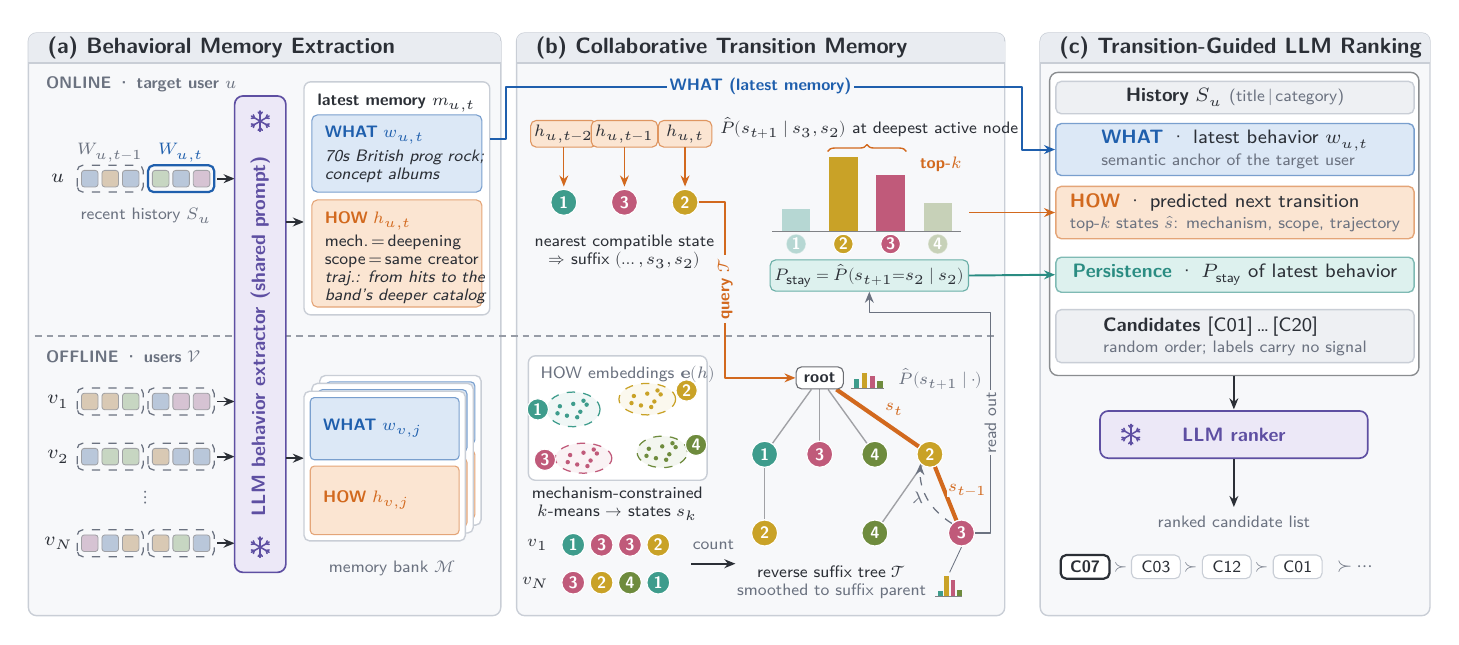
\begin{tikzpicture}[font=\lsz,text=ink,line join=round]

% =====================================================================
% PANELS
% =====================================================================
\begin{pgfonlayer}{background}
\foreach \x/\X/\t in {0/6.0/{(a) Behavioral Memory Extraction},
                      6.2/12.4/{(b) Collaborative Transition Memory},
                      12.85/17.8/{(c) Transition-Guided LLM Ranking}}{
  \draw[panelbox] (\x,0) rectangle (\X,7.4);
  \begin{scope}
    \clip[rounded corners=3pt] (\x,0) rectangle (\X,7.4);
    \fill[band] (\x,7.02) rectangle (\X,7.4);
  \end{scope}
  \draw[rule,line width=0.5pt] (\x,7.02) -- (\X,7.02);
  \node[font=\hsz\bfseries,anchor=west] at (\x+0.12,7.21) {\t};
}
\end{pgfonlayer}
% online / offline separator across (a) and (b)
\draw[mute!70,dash pattern=on 2.5pt off 1.8pt,line width=0.5pt] (0.08,3.55) -- (12.32,3.55);
\node[anchor=north west,font=\tsz\bfseries,text=mute] at (0.1,6.97) {ONLINE\,\,·\,\,target user $u$};
\node[anchor=north west,font=\tsz\bfseries,text=mute] at (0.1,3.49) {OFFLINE\,\,·\,\,users $\mathcal{V}$};

% =====================================================================
% (a) BEHAVIORAL MEMORY EXTRACTION
% =====================================================================
% item positions inside a window-of-3 layout
\def\ix#1{\fpeval{0.78+0.26*#1+(#1>2)*0.12}}

% ---- online: target user history ----
\def\yy{5.55}
\node[font=\lsz\itshape] at (0.38,\yy) {$u$};
\foreach \i/\c in {0/iA,1/iB,2/iA,3/iC,4/iA,5/iD}{
  \node[item,fill=\c] at (\ix{\i},\yy) {};
}
\draw[win] (\ix{0}-0.16,\yy-0.17) rectangle (\ix{2}+0.16,\yy+0.17);
\draw[draw=what,rounded corners=2pt,line width=0.8pt] (\ix{3}-0.16,\yy-0.17) rectangle (\ix{5}+0.16,\yy+0.17);
\node[font=\tsz,text=mute] at ({(\ix{0}+\ix{2})/2},\yy+0.33) {$W_{u,t-1}$};
\node[font=\tsz,text=what] at ({(\ix{3}+\ix{5})/2},\yy+0.33) {$W_{u,t}$};
\node[font=\tsz,text=mute,anchor=north] at ({(\ix{0}+\ix{5})/2},\yy-0.24) {recent history $S_u$};
\draw[flow] (\ix{5}+0.2,\yy) -- (2.62,\yy);

% ---- offline: training users ----
\foreach \u/\yy/\cs in {{v_1}/2.72/{iB,iB,iC,iA,iD,iD},{v_2}/2.02/{iA,iC,iC,iB,iA,iA},{v_N}/0.92/{iD,iA,iB,iB,iC,iA}}{
  \node[font=\lsz\itshape] at (0.38,\yy) {$\u$};
  \foreach \c [count=\j from 0] in \cs { \node[item,fill=\c] at (\ix{\j},\yy) {}; }
  \draw[win] (\ix{0}-0.16,\yy-0.17) rectangle (\ix{2}+0.16,\yy+0.17);
  \draw[win] (\ix{3}-0.16,\yy-0.17) rectangle (\ix{5}+0.16,\yy+0.17);
  \draw[flow] (\ix{5}+0.2,\yy) -- (2.62,\yy);
}
\node[text=mute] at ({(\ix{0}+\ix{5})/2},1.5) {$\vdots$};

% ---- shared LLM extractor ----
\draw[draw=llm,fill=llmbg,rounded corners=3pt,line width=0.6pt] (2.62,0.55) rectangle (3.27,6.6);
\node[rotate=90,font=\lsz\bfseries,text=llm] at (2.945,3.55) {LLM behavior extractor (shared prompt)};
\snow{(2.945,6.28)}{llm}
\snow{(2.945,0.87)}{llm}

% ---- online: example memory card ----
\draw[flow] (3.27,5.0) -- (3.5,5.0);
\begin{scope}
  \draw[rule,fill=white,rounded corners=2.5pt,line width=0.5pt] (3.5,3.82) rectangle (5.86,6.78);
  \node[anchor=north west,font=\tsz\bfseries] at (3.55,6.75) {latest memory $m_{u,t}$};
  % WHAT band
  \draw[draw=what!60,fill=whatbg,rounded corners=2pt,line width=0.4pt] (3.6,5.38) rectangle (5.76,6.36);
  \node[anchor=north west,font=\tsz\bfseries,text=what] at (3.64,6.34) {WHAT\,\,$w_{u,t}$};
  \node[anchor=north west,font=\tsz,align=left,text=ink] at (3.64,6.04) {\itshape 70s British prog rock;\\[-0.5pt]\itshape concept albums};
  % HOW band
  \draw[draw=how!60,fill=howbg,rounded corners=2pt,line width=0.4pt] (3.6,3.92) rectangle (5.76,5.28);
  \node[anchor=north west,font=\tsz\bfseries,text=how] at (3.64,5.26) {HOW\,\,$h_{u,t}$};
  \node[anchor=north west,font=\tsz,align=left,text=ink] at (3.64,4.96)
     {mech.\,=\,deepening\\[-0.5pt]scope\,=\,same creator\\[-0.5pt]\itshape traj.: from hits to the\\[-0.5pt]\itshape band's deeper catalog};
\end{scope}

% ---- offline: memory bank ----
\draw[flow] (3.27,2.0) -- (3.5,2.0);
\foreach \k in {2,1,0}{
  \begin{scope}[shift={(0.1*\k,0.1*\k)}]
    \draw[rule,fill=white,rounded corners=2pt,line width=0.5pt] (3.5,0.95) rectangle (5.55,2.85);
    \draw[draw=what!60,fill=whatbg,rounded corners=1.5pt,line width=0.4pt] (3.58,1.98) rectangle (5.47,2.77);
    \draw[draw=how!60,fill=howbg,rounded corners=1.5pt,line width=0.4pt] (3.58,1.03) rectangle (5.47,1.9);
  \end{scope}
}
\node[anchor=west,font=\tsz\bfseries,text=what] at (3.62,2.38) {WHAT $w_{v,j}$};
\node[anchor=west,font=\tsz\bfseries,text=how]  at (3.62,1.47) {HOW $h_{v,j}$};
\node[font=\tsz,text=mute] at (4.62,0.6) {memory bank $\mathcal{M}$};

% =====================================================================
% (b) COLLABORATIVE TRANSITION MEMORY
% =====================================================================
% ---------------- offline: HOW embedding space + states ----------------
\draw[rule,fill=white,rounded corners=2.5pt,line width=0.5pt] (6.35,1.72) rectangle (8.62,3.3);
\node[anchor=north west,font=\tsz,text=mute] at (6.38,3.29) {HOW embeddings $\mathbf{e}(h)$};
\foreach \cx/\cy/\c/\lab/\rx/\ry in {6.92/2.62/sA/1/0.34/0.22, 7.86/2.75/sB/2/0.36/0.2, 7.05/2.0/sC/3/0.36/0.19, 8.05/2.08/sD/4/0.32/0.2}{
  \draw[\c,dashed,line width=0.45pt,fill=\c!8] (\cx,\cy) ellipse ({\rx} and {\ry});
  \foreach \dx/\dy in {-0.17/0.04,-0.08/-0.08,0.0/0.07,0.09/-0.03,0.17/0.06,0.05/-0.1,-0.2/-0.05,0.13/0.11}{
    \fill[\c] (\cx+\dx,\cy+\dy) circle (0.028);
  }
}
\node[st,fill=sA,minimum size=0.27cm] at (6.47,2.62) {1};
\node[st,fill=sB,minimum size=0.27cm] at (8.36,2.86) {2};
\node[st,fill=sC,minimum size=0.27cm] at (6.56,1.98) {3};
\node[st,fill=sD,minimum size=0.27cm] at (8.48,2.17) {4};
\node[font=\tsz,text=ink,align=center] at (7.48,1.42) {mechanism-constrained\\[-0.5pt]$k$-means $\to$ states $s_k$};

% state sequences of training users
\def\sq#1#2#3{%
  \node[font=\tsz\itshape,anchor=east] at (6.72,#2) {$#1$};
  \foreach \c/\n [count=\j from 0] in {#3}{ \node[st,fill=\c,minimum size=0.29cm] at (6.92+0.36*\j,#2) {\n}; }
}
\sq{v_1}{0.9}{sA/1,sC/3,sC/3,sB/2}
\sq{v_N}{0.42}{sC/3,sB/2,sD/4,sA/1}
\draw[flow] (8.42,0.66) -- (8.98,0.66);
\node[font=\tsz,text=mute,align=center] at (8.7,0.9) {count};

% ---------------- offline: reverse suffix tree ----------------
\node[draw=ink!70,fill=white,rounded corners=2pt,font=\tsz\bfseries,minimum width=0.6cm,minimum height=0.28cm,inner sep=1pt] (root) at (10.05,3.02) {root};
\st{n1}{(9.35,2.05)}{sA}{1}
\st{n3}{(10.05,2.05)}{sC}{3}
\st{n4}{(10.75,2.05)}{sD}{4}
\st{n2}{(11.45,2.05)}{sB}{2}
\st{n12}{(9.35,1.05)}{sB}{2}
\st{n24}{(10.75,1.05)}{sD}{4}
\st{n23}{(11.85,1.05)}{sC}{3}
\begin{pgfonlayer}{background}
  \foreach \a/\b in {root/n1,root/n3,root/n4,n1/n12,n2/n24}{ \draw[ink!45,line width=0.5pt] (\a) -- (\b); }
  \draw[how,line width=1.5pt] (root) -- (n2);
  \draw[how,line width=1.5pt] (n2) -- (n23);
\end{pgfonlayer}
\node[font=\tsz,text=how,fill=panel,inner sep=0.5pt] at (11.0,2.62) {$s_t$};
\node[font=\tsz,text=how,fill=panel,inner sep=0.5pt] at (11.93,1.6) {$s_{t-1}$};
% node-level next-state distributions
\hist{(10.48,2.88)}{0.12}{0.2}{0.16}{0.1}{0.075}
\node[font=\tsz,text=mute,anchor=west] at (10.93,3.0) {$\hat P(s_{t+1}\mid\cdot)$};
\hist{(11.55,0.25)}{0.06}{0.26}{0.2}{0.08}{0.06}
\draw[mute,line width=0.3pt] (11.85,0.87) -- (11.7,0.55);
% suffix-parent smoothing
\draw[->,dashed,mute,line width=0.45pt] (n23.north west) to[bend left=30] node[pos=0.5,left,font=\tsz,text=mute,inner sep=1pt] {$\lambda$} (n2.south west);
\node[font=\tsz,text=ink,align=center] at (10.2,0.42) {reverse suffix tree $\mathcal{T}$\\[-0.5pt]\textcolor{mute}{smoothed to suffix parent}};

% ---------------- online: map target memories to states ----------------
\foreach \x/\lab in {6.8/{t-2},7.57/{t-1},8.34/{t}}{
  \node[chip,draw=how!70,fill=howbg,minimum width=0.68cm] at (\x,6.12) {$h_{u,\lab}$};
  \draw[->,line width=0.5pt,draw=how] (\x,5.95) -- (\x,5.45);
}
\st{q1}{(6.8,5.25)}{sA}{1}
\st{q3}{(7.57,5.25)}{sC}{3}
\st{q2}{(8.34,5.25)}{sB}{2}
\node[font=\tsz,align=center,text=ink] at (7.57,4.62) {nearest compatible state\\[-0.5pt]$\Rightarrow$ suffix $(\dots,s_3,s_2)$};

% query: walk reversed suffix from the root
\draw[flow,draw=how] (q2.east) -- (8.85,5.25) -- (8.85,3.02) -- (root.west);
\node[font=\tsz\bfseries,text=how,rotate=90,fill=panel,inner sep=1pt] at (8.85,4.15) {query $\mathcal{T}$};

% ---------------- online: read-out distribution ----------------
\node[font=\tsz,anchor=south] at (10.68,5.93) {$\hat P(s_{t+1}\mid s_3,s_2)$ at deepest active node};
\def\bw{0.36}
\foreach \c/\h/\n/\x/\op in {sA/0.28/1/9.75/0.35, sB/0.95/2/10.35/1, sC/0.72/3/10.95/1, sD/0.36/4/11.55/0.35}{
  \fill[\c,opacity=\op] (\x-\bw/2,4.88) rectangle (\x+\bw/2,4.88+\h);
  \node[st,fill=\c,minimum size=0.25cm,opacity=\op,text opacity=1] at (\x,4.72) {\n};
}
\draw[ink!60,line width=0.35pt] (9.45,4.88) -- (11.85,4.88);
\draw[decorate,decoration={brace,amplitude=2.5pt,raise=1pt},how,line width=0.5pt] (10.15,5.86) -- (11.15,5.86);
\node[font=\tsz\bfseries,text=how,anchor=west] at (11.2,5.73) {top-$k$};
% persistence
\node[chip,draw=stay!70,fill=staybg,text=ink,anchor=center] (pst) at (10.68,4.32) {$P_{\text{stay}}=\hat P(s_{t+1}{=}s_2\mid s_2)$};
% read-out arrow from tree
\draw[->,line width=0.5pt,draw=mute] (n23.east) -- (12.22,1.05) -- (12.22,3.85) -- (pst.south |- 0,3.85) -- (pst.south);
\node[font=\tsz,text=mute,rotate=90,fill=panel,inner sep=0.6pt] at (12.22,2.45) {read out};

% =====================================================================
% (c) TRANSITION-GUIDED LLM RANKING
% =====================================================================
\draw[draw=ink!55,fill=white,rounded corners=3pt,line width=0.5pt] (12.97,3.05) rectangle (17.66,6.9);
\node[slot,draw=rule,fill=histbg] (p1) at (13.04,6.58)
  {\textbf{History} $S_u$ \textcolor{mute}{\tsz(title\,|\,category)}};
\node[slot,draw=what!60,fill=whatbg,text=ink] (p2) at (13.04,5.92)
  {\textcolor{what}{\textbf{WHAT}} · latest behavior $w_{u,t}$\\[-0.5pt]{\tsz\textcolor{mute}{semantic anchor of the target user}}};
\node[slot,draw=how!60,fill=howbg,text=ink] (p3) at (13.04,5.12)
  {\textcolor{how}{\textbf{HOW}} · predicted next transition\\[-0.5pt]{\tsz\textcolor{mute}{top-$k$ states $\hat s$: mechanism, scope, trajectory}}};
\node[slot,draw=stay!60,fill=staybg,text=ink] (p4) at (13.04,4.33)
  {\textcolor{stay}{\textbf{Persistence}} · $P_{\text{stay}}$ of latest behavior};
\node[slot,draw=rule,fill=histbg] (p5) at (13.04,3.55)
  {\textbf{Candidates} [C01]\,\dots\,[C20]\\[-0.5pt]{\tsz\textcolor{mute}{random order; labels carry no signal}}};

% incoming evidence
\draw[flow,draw=what] (5.86,6.05) -- (6.06,6.05) -- (6.06,6.72) -- (12.62,6.72) -- (12.62,5.92) -- (p2.west);
\node[font=\tsz\bfseries,text=what,fill=panel,inner sep=0.8pt] at (9.3,6.72) {WHAT (latest memory)};
\draw[flow,draw=how] (11.95,5.12) -- (p3.west);
\draw[flow,draw=stay] (pst.east) -- (p4.west);

% ranker
\draw[flow] (15.31,3.05) -- (15.31,2.62);
\node[draw=llm,fill=llmbg,rounded corners=3pt,line width=0.6pt,minimum width=3.4cm,minimum height=0.6cm,font=\lsz\bfseries,text=llm] (rk) at (15.31,2.3) {LLM ranker};
\snow{(14.0,2.3)}{llm}
\draw[flow] (rk.south) -- (15.31,1.38);

% ranked output
\node[font=\tsz,text=mute,anchor=south] at (15.31,1.0) {ranked candidate list};
\foreach \lab/\x [count=\r] in {C07/13.42,C03/14.32,C12/15.22,C01/16.12}{
  \ifnum\r=1
    \node[chip,draw=ink,fill=white,line width=0.8pt,font=\tsz\bfseries,minimum width=0.62cm] (o\r) at (\x,0.62) {\lab};
  \else
    \node[chip,draw=rule,fill=white,minimum width=0.62cm] (o\r) at (\x,0.62) {\lab};
  \fi
}
\foreach \a/\b in {1/2,2/3,3/4}{ \node[font=\tsz,text=mute] at ($(o\a)!0.5!(o\b)$) {$\succ$}; }
\node[font=\lsz,text=mute] at (16.85,0.62) {$\succ\cdots$};

\end{tikzpicture}
\end{document}
